\documentclass[xcolor=dvipsnames]{beamer}
\usepackage{xmpmulti}
\usepackage{comp2402}

\title{Priority Queues, Heaps, and HeapSort}
\author{}
\date{}


\begin{document}

\begin{frame}
  \titlepage
  \begin{center}
    
\includegraphics[height=1.2in]{images/heap.jpg}
  \end{center}
\end{frame}

\begin{frame}
  \frametitle{Priority queues}
  \begin{itemize}
    \item<1->A \emph{priority queue} stores a collection of #Comparable# elements
    \item<2->Operations:
    \begin{itemize}
      \item<3-> #add(x)# : Add #x# to the collection
      \item<4-> #findMin()# : Return the smallest element in the collection
      \item<5-> #deleteMin()# : Remove the smallest element in the collection
    \end{itemize}
    \item<6-> In the JCF Queue interface, these are:
    \begin{itemize}
      \item #add(x)/offer(x)# : #add(x)#
      \item #peek()# : #findMind()#
      \item #remove()/poll()# : #deleteMin()#
    \end{itemize}
  \end{itemize}
\end{frame}

\begin{frame}[fragile]
  \frametitle{Application 1: Sorting}

  \begin{itemize}
    \item We can sort a set of elements by inserting them all into a priority queue and then removing them  
  \end{itemize}
\begin{lstlisting}
  public static <T> void sort(T[] a) {
    Queue<T> pq = new PriorityQueue<T>();
    for (T x : a) 
      pq.add(x);
    for (int i = 0; i < a.length; i++)
      a[i] = pq.remove();
  }
\end{lstlisting}
\end{frame}

\begin{frame}[fragile]
  \frametitle{Application 2: Queueing systems}

\begin{lstlisting}
class Packet implements Comparable<Packet> {
  int compareTo(Packet p) {
    return this.priority - p.priority;
  }
  ...
}
class NetworkSwitch {
  public void receive(Packet p) {
    pq.add(p);
  }
  ...
  public void sendNext() {
    send(pq.remove());
  }
}
\end{lstlisting}
\end{frame}

\begin{frame}
  \frametitle{Application 3: Simulation}
 
  \begin{itemize}
    \item<1->In simulations, priority queues store events ordered by time of occurrence
  \end{itemize}
  \multiinclude[<+>][start=1,format=pdf,width=3in]{figs/sim}
\end{frame}

\begin{frame}
  \frametitle{Heaps}
  \begin{itemize}
    \item<1-> Priority queues can be implemented as (binary) \emph{heaps}
    \item<2-> A binary heap is a binary tree where each node #u# stores a value #u.prio#
    \begin{itemize}
      \item<3-> Heap property: #u.prio < u.left.prio# and #u.prio < u.right.prio#
    \end{itemize}
  \end{itemize}
  \begin{center}
    
\includegraphics{sfigs/heap}
  \end{center}
\end{frame} 


\begin{frame}
  \frametitle{Complete binary heaps}
  \begin{itemize}
    \item<1-> A \emph{complete} heap uses a complete binary tree:
    \begin{itemize}
      \item<2->A complete binary tree of height $d$ has up to $2^{d+1}-1$ nodes
      \item<3->To store $n$ nodes, we require $2^{d+1}-1 \ge #n#$
      \begin{itemize}
        \item<4->$2^{d+1} \ge #n#+1$
        \item<5->$d+1 \ge \log(#n#+1)$
        \item<6->$d \ge \log(#n#+1)-1\only<7->{= O(\log #n#)}$
      \end{itemize}
      \item[] \begin{center}
\includegraphics[width=2.5in]{sfigs/heap}\end{center}
    \end{itemize}
    \item<7-> A complete heap of size $#n#$ has height $O(\log #n#)$
  \end{itemize}
  \end{frame} 


\begin{frame}
  \frametitle{Ahnentafel lists}
 
  \begin{itemize}
    \item<1->The \emph{Eytzinger method} maps the nodes of a complete binary tree to the positions of an array #a#
    \begin{itemize}
      \item<2-> #a[0]# is the root
      \item<3-> the left child of #a[i]# is #a[2*i+1]#
      \item<4-> the right child of #a[i]# is #a[2*i+2]#
      \item<5-> the parent #a[i]# is #a[(i-1)/2]#
    \end{itemize}
    \item[]\begin{center}\begin{tabular}{cc}
             \includegraphics[height=1.2in]{sfigs/ahnentafel}&
             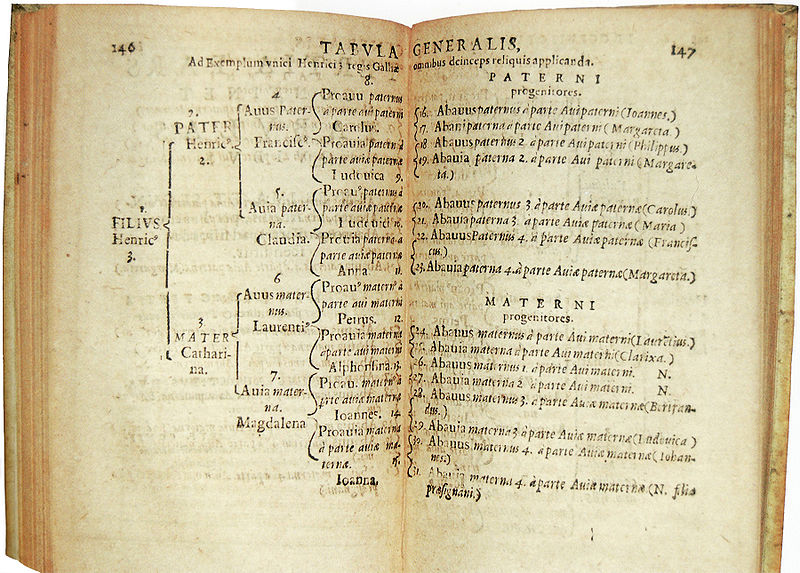
\includegraphics[height=1.2in]{images/eytzinger}
           \end{tabular}\end{center}
  \end{itemize}
\end{frame}

\begin{frame}[fragile]
  \frametitle{Implicit binary heaps}

  \begin{itemize}
    \item<1->An \emph{implicit binary heap} represents a complete binary heap in an array #a# using the Eytzinger method
    \item<2->[]\begin{center}\includegraphics[width=2.5in]{sfigs/binheap}\end{center}
    \item<3-> No extra pointers, all the data lives in #a#
  \end{itemize}
\end{frame} 


\begin{frame}[fragile]
\javaimport{ods/BinaryHeap.a.n.left(i).right(i).parent(i)}
\end{frame}


\begin{frame}[fragile]
  \frametitle{Finding the min}

  \begin{itemize}
    \item<1->Finding the minimum value in a heap is easy
    \begin{itemize}
      \item<2->It's stored at the root
      \item<3->This is #a[0]#
    \end{itemize}
    \item<4->[]
    \javaimport{ods/BinaryHeap.peek()}
    \item<5->Runs in $O(1)$ time
  \end{itemize}
\end{frame}


\begin{frame}
  \frametitle{Inserting into a heap}

  \begin{itemize}
    \item<1->To insert #x# into a (implicit binary) heap, we
    \begin{enumerate}
      \item<2->add #x# as a leaf
      \item<3->while #x# is smaller than #parent(x)#
      \begin{itemize}
        \item<4-> swap #x# with its parent
      \end{itemize}

    \end{enumerate}
    \item[]\begin{center}
      \includegraphics[width=2.5in]{sfigs/binheap}
    \end{center}
    \item<5->Runs in $O(\log #n#)$ time
  \end{itemize}
\end{frame} 



\begin{frame}[fragile]
\javaimport{ods/BinaryHeap.add(x).bubbleUp(i)}
\end{frame}



\begin{frame}
  \frametitle{Deleting from a heap}
  \begin{itemize}
    \item<1->To delete the min from a heap, we
    \begin{enumerate}
      \item<2->copy #x=a[n-1]# into #a[0]#
      \item<3->while #x# is larger than either of its children
      \begin{itemize}
        \item<4-> swap #x# with the smaller of its children
      \end{itemize}
    \end{enumerate}
    \item[]\begin{center}
      \includegraphics[width=2.5in]{sfigs/binheap}
    \end{center}
    \item<5->Runs in $O(\log #n#)$ time
  \end{itemize}
\end{frame}

\begin{frame}[fragile]
\javaimport{ods/BinaryHeap.remove()}
\end{frame}

\begin{frame}[fragile]
\javaimport{ods/BinaryHeap.trickleDown(i)}
\end{frame}

\begin{frame}
  \frametitle{Summary so far}

  \begin{itemize}
    \item \textbf{Theorem:} A (implicit) binary heap supports the operations #add(x)# and #deleteMin()# in $O(\log #n#)$ (amortized) time and supports the #findMin()# operation in $O(1)$ time.
  \end{itemize} 
\end{frame}




\begin{frame}[fragile]
  \frametitle{Building a heap}
 
  \begin{itemize}
    \item<+-> Suppose we are given an unsorted array #a#
    \item<+-> How quickly can we make #a# into an implicit binary heap?
    \item<+-> We can insert elements #a[0],...,a[n-1]# one at a time
\begin{lstlisting}
  public BinaryHeap(T[] ia) {
    a = ia;
    for (int n = 1; n < a.length; n++) {
      add(a[n]);
    }
  }
\end{lstlisting}
    \item<+-> This takes $O(1+\log(1)) + O(1+\log(2)) + \cdots O(1+\log #n#)$ time
    \item<+-> ${}= O(#n#\log #n#)$
    \item<+-> Can we do better?
  \end{itemize}
\end{frame}



\begin{frame}[fragile]
  \frametitle{Building a heap in linear time}
 
  \begin{itemize}
    \item<+-> We can do better by working bottom up
    \item<+-> First build $\approx #n#/2$ heaps of size 1
    \item<+-> Next, build $\approx #n#/4$ heaps of size 3
    \item<+-> Next, build $\approx #n#/8$ heaps of size 7
    \item<+-> \ldots
    \item<+-> Build $1$ heap of size $#n#$
    \item<+->[]
    \javaimport{ods/BinaryHeap.BinaryHeap(a,c)}
  \end{itemize}
\end{frame}



\begin{frame}
  \frametitle{Building a heap in linear time - analysis}

  \begin{itemize}
    \item<1-> We call #trickleDown(i)# $n/2^{j}$ times when $#i#$ is the root of heap of size $2^j-1$
    \item<2-> #trickleDown(i)# then takes $O(\log (2^j-1)) = O(j)$ time
    \item<3-> Total running time is
    \begin{itemize}
      \item<4->$(#n#/4)\cdot O(1)$
      \item<5->$(#n#/8)\cdot O(2)$
      \item<6->$(#n#/16)\cdot O(3)$
      \item<7->\ldots
      \item<8->$1\cdot O(\log #n#)$
      \item<9->${} = O(#n#)$\footnote{exercise: prove this}
    \end{itemize}
  \end{itemize}
\end{frame}


\begin{frame}[fragile]
  \frametitle{Heapsort}

  \begin{itemize}
    \item<1->The heapsort algorithm for sorting an array #a# of length $#n#$:
    \item<2->Make #a# into a heap in ($O(#n#)$ time)
    \item<3->Repeat $#n#$ times:
    \begin{itemize}
      \item<4->Delete the minimum
    \end{itemize}
    \item<5->[]
    \javaimport{ods/BinaryHeap.sort(a,c)}
    \item<6->Each deletion takes $O(\log n)$ time
    \item<7->Runs in $O(n\log n)$ time
    \item<8->Doesn't require any extra space --- does all work inside of input array #a#
  \end{itemize}
\end{frame}

\end{document}

\end{document}

